% Chapter 1

\chapter{Neutron Measurements at IP2I cryogenic facility} % Main chapter title

\label{ChapterNeutron} % Change X to a consecutive number; for referencing this chapter elsewhere, use \ref{ChapterX}

%----------------------------------------------------------------------------------------
%	BEGING CHAPTER

\underline{PERSONNAL REF}
{\color{red}[see Neutron measurements at IP2I with Ge
bolometers.pdf]}

\href{https://elog.ipnl.in2p3.fr/manoir/R%26D+Cryo+LIO/51}{https://elog.ipnl.in2p3.fr/manoir/R\%26D+Cryo+LIO/51}

\underline{WEAK REF}

{\color{red}[see NeutronMeasurementCampaign.pdf]}

OFNote.pdf

\underline{STRONG REF}

68Ge-68Ga-Decay.pdf


%----------------------------------------------------------------------------------------


\section{Motivation}

As the Ricochet experiment is happening near a nuclear reactor, there is a risk that the bolometers will be blinded by the radioactive background of the site.
The radioactive background is mainly composed of particles inducing electronic recoil (such as gammas, electrons, muons, charged particles essentially) and neutron producing neutron recoil.
While the former background component can be discriminated thanks to technology used in the bolometers, the latter can not and thus constitute an unavoidable background for Ricochet which will limit the CENNS process measurement.
Therefore, it is vital to evaluate the neutron background on-site and understand its dependency in the energy.
In addition to estimating the limitations on the measurement, the study of the neutron background on-site will also be used in the design of the shielding.

\begin{figure}
\centering
\begin{subfigure}{.5\textwidth}
  \centering
  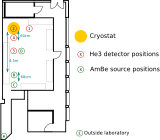
\includegraphics[width=\linewidth]{Figures/Neutron/scheme_ip2i.png}
  \caption{IP2I: R\&D Laboratory}
  \label{fig:scheme-ill}
\end{subfigure}%
\begin{subfigure}{0.5\textwidth}
  \centering
  \includegraphics[width=\linewidth]{Figures/Neutron/scheme_ill.png}
  \caption{ILL: Reactor Site}
  \label{fig:scheme-ip2i}
\end{subfigure}
\caption{Schemes of the neutron background measurements site with \ce{^3He} gaseous detectors. The positions of the detectors and the neutron source are indicated with numbered/colored tokens.}
\label{fig:scheme-site}
\end{figure}

The actual measurement of the neutron background at the ILL site \ref{fig:scheme-ill} was achieved with gaseous Helium-3 Tube Detector based on the neutron capture by \ce{^3He}:

\begin{equation}
	\ce{^1_0n + ^3He -> ^3H + ^1_1p}
\end{equation}

This detector technology is sensitive to thermal/fast? neutron at high energy >MeV which is order of magnitude superior to the energy range of the cryogenic germanium bolometers.
The estimation of the neutron background at ILL in the energy range of interest is then obtained by extrapolation of the neutron background at IP2I validated with relative measurements between the tube detector and the germanium detector technology.


\section{Experimental Setup}

The measure of the neutron background at the IP2I cryogenic facility was done with a newly designed low-threshold germanium detector of the RED series called RED80 with RMS resolution of approximately 120eV on the heat channel and 200eV on the ionization channel.
The data were taken during the run 57 which began on 03/07/2019 and ended on 01/08/2019. In this run, RED80 and RED70 were both operated on the suspended tower.

\begin{figure}
\centering
\begin{subfigure}{.5\textwidth}
  \centering
  \includegraphics[width=\linewidth]{Figures/Neutron/photo_red80.png}
  \caption{Photo of RED80}
  \label{fig:photo-red80}
\end{subfigure}%
\begin{subfigure}{0.5\textwidth}
  \centering
  \includegraphics[width=\linewidth]{Figures/Neutron/scheme_red80.png}
  \caption{Scheme of RED80}
  \label{fig:scheme-red80}
\end{subfigure}
\caption{Description of RED80, with a schematic drawing of the Germanium crystal, the NTD sensor and the position and polarization of the electrodes.}
\label{fig:description-red80}
\end{figure}

% Description of RED80
RED80 is composed of a 38g cylindrical germanium crystal of height 10mm and diameter 30mm.
It is equipped with a heat channel and an ionization channel (see figure \ref{fig:description-red80})
The ionization channel consists of a pair of collecting electrodes and guard electrodes.
The collecting electrodes are two flat full aluminium electrodes of diameter 27mm deposited on its top and bottom surface.
The guard electrodes are four circular electrodes deposited on its side.
The heat channel consists of a NTDGe thermistance labeled K58 with dimension 4*4*0.45 mm.
Before being installed into the cryostat, the detector was place near a neutron source in order to activate the Germanium crystal and benefit from the intrinsic gamma calibration peak during operation. The neutron activation started on 28/06/2019 at 17h08 and ended on 02/08/2019 at 10h08 yielding 89h of activation.

% Conditions of data taking
From 08/08/2019, the detectors were characterized at 18mK. As for the actual condition of the neutron background measuremets, RED80 was operated at 16mK with an optimal NTD polarization current of 1nA and an electric potential difference of 2V on the ionization channel:
$$ A, B, C, D = +1, +1, -1, -1.$$

The data taking was divided between two configurations, "Background" and "Calibration", meant to measure the neutron background and calibrate the neutron recoil band in the detector respectively.
The Background configuration was used to save 34 hours of data partitioned in three streams: tg18l005, tg27l000 and tg28l000.
The Calibration configurations was used to take 78 hours of data, with an Americium-Beryllium neutron source situated 4.5m away from the cryostat and shielded with milk (acting as water) to thermalize the emitted neutron (see figure ??). The data were saved in four streams: tg17l007, tg19l010, tg20l000 and tg21l000.

\begin{figure}
\centering
\begin{subfigure}{.5\textwidth}
  \centering
  \includegraphics[width=\linewidth]{Figures/Neutron/photo_source_front.jpg}
  \caption{Front view, towards the cryostat}
  \label{fig:photo-source-frontt}
\end{subfigure}%
\begin{subfigure}{0.5\textwidth}
  \centering
  \includegraphics[width=\linewidth, angle=-90]{Figures/Neutron/photo_source_rear.jpg}
  \caption{Rear view}
  \label{fig:photo-source-rear}
\end{subfigure}
\caption{Photo of the shielded AmBe neutron source used for the neutron calibration.}
\label{fig:photo-source}
\end{figure}

Each stream was taken during nights or week-ends to benefit from the long time with stable operation (see Table \ref{tab:neutron-streams}). The configurations were mixed in term of dates, which is of importance when measuring the rate of the Germanium calibration peaks which is decreasing with time.

\begin{table}[]
\centering
\begin{tabular}{l|l|r}
Configuration                & Stream   & Started at          \\ \hline
\multirow{3}{*}{Background}  & tg18l005 & ?? on 18/08/2019    \\
                             & tg27l000 & 21h20 on 27/08/2019 \\
                             & tg28l000 & 11h27 on 28/08/2019 \\ \hline
\multirow{4}{*}{Calibration} & tg17l007 & ?? on 17/08/2019    \\
                             & tg19l010 & 17h10 on 19/08/2019 \\
                             & tg20l000 & ?? on 20/08/2019    \\
                             & tg21l000 & ?? on 21/08/2019   
\end{tabular}
\caption{Starting hours and date of the streams for neutron background and calibration measurements.}
\label{tab:neutron-streams}
\end{table}


\section{Data Analysis}


\subsection{Pre-processing and Data format}
\label{par:data-format}

The data were initially saved as streams: the voltage value of the heat channel and the four ionization channel are saved for each time step in the acquisition with a sampling frequency of 400Hz. 

{\color{red} FIGURE STREAM HEAT/IONIZATION}

These voltage values are extracted by an analog-to-digital conversion system and thus expressed in \textbf{A}nalog-to-\textbf{D}igital conversion \textbf{U}nit (ADU).
These data streams are then processed by an \textbf{O}ptimal \textbf{F}iltering (OF) software called NEPAL developed by Julien Billard. A filter based on the signal PSD and the noise PSD in the bolometer is applied to the stream. Time windows of 1s centered on a triggering events are selected with an amplitude threshold on the filtered stream (see Figure \ref{fig:pulse-of}).

\begin{figure}
\centering
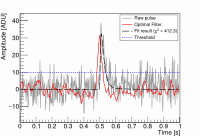
\includegraphics[width=\linewidth,]{Figures/Neutron/pulse_of.png}
\caption{Optimal filtering of a 1s pulse window.}
\label{fig:pulse-of}
\end{figure}

These time windows are processed to extract several quantities:
\begin{itemize}
	\item Timestamp,
	\item Amplitude (filtered decorrelated),
	\item Chi2 value (filtered decorrelated),
	\item Offset (raw),
	\item Ionization Slope (raw),
\end{itemize}
The figure \ref{fig:analysis-monitoring-demo} shows this characterization quantities for each triggering event as a function of their timestamp (for the considered stream, here tg17l007). Each scatter plots is understood when applying the quality cut:
\begin{itemize}
	\item Heat Energy vs Timestamp: Reconstruction of the energy deposited in the heat channel for each event. This graph can be linked to the heat energy spectrum presented later. One can note pronounced population of fixed energy corresponding to the abundance of 10.37keV events due to the activation of the Germanium crystal and the noise blob poulation at $\mathcal{O}(50)$eV.
	\item Ionization Energy vs Timestamp: is quite the same as heat energy, except that with the overlap of the different channels this graph is now an useless mess
	\item Offset Heat vs Timestamp: this curve is proportional to the resistance value of the NTD sensor and allows us to follow the baseline temperature. With this decreasing profile, we deduce that the detector has been cooling during this stream. Note that although RED80 is still slowly thermalizing, the sensitivity is stable (precision?)
	\item Offset Ionization vs Timestamp: this curve is essentially used to discard all the events with an offset outside of the $[-14000, 14000]$ ADU (see \ref{par:quality-cuts}).
	\item Slope Ionization vs Timestamp: this curve is proportional to the baseline current measured by each electrodes. This baseline current is explained by the presence of leakage current between the electrodes (dedicated section?) and the collection of trapped charges (especially after a maintenance).
	\item Chi2 vs Timestamp: This describes the goodness of the fit of the template to the pulse. A stable low value indicate a fixed shape for the pulses, which is required for the chi2 cut applied later (see \ref{par:quality-cuts})
\end{itemize}

\begin{figure}
\centering
\includegraphics[width=\linewidth,]{Figures/Neutron/analysis_monitoring_demo.png}
\caption{Characterization quantities of triggering events as a function of their timestamp. (TO BE CHANGE !)}
\label{fig:analysis-monitoring-demo}
\end{figure}

In the end, for each configuration of data measurements(Background and Calibration), triggering events were selected in each streams and described by several quantities.
Among those triggering events are events of interest well reconstructed and induced by electronic recoil from the radioactive gamma background, the KLM activation lines from the germanium and the cosmic muons and neutron recoil from the AmBe neutron source and the radioactive neutron background. However, many triggering events can not be reconstructed or were induced by parasitic source, and can not yield information for the measurement of the neutron background at IP2I. To extract the events of interest from all the data, analysis cuts are applied.


\subsection{Glitch Time Cut}

{\color{red} We should also substract the maintenance time ?}

Some portions of the streams are glitched for reasons not clearly understood relative to the acquisition electronics or the cryostat temperature regulation system (see figure \ref{}).

\begin{figure}
\centering
\includegraphics[width=\linewidth,]{Figures/Neutron/analysis_glitch_cut_demo.png}
\caption{Heat Amplitude in function of the Timestamp. All events are in grey, while events passing the "Glitch Time Cut" are in blue.}
\label{fig:analysis-monitoring-demo}
\end{figure}

Thus, some time intervals were chosen for each streams where the events would not pass what is called the "Glitch Time Cut" (see table \ref{tab:stream-glitch-time-cut}). It is important to consider the appropriate livetime. Indeed, all the results presented later will be weighted by the exposure of the detector. Thus, period of time when the detector is not available for proper measurements should be discarded from the analysis and not taken into the computation of the exposure.

\begin{table}[]
\centering
\resizebox{\linewidth}{!}{
	\begin{tabular}{l|cc|r|r|r|l|r}
\multicolumn{1}{c|}{\multirow{2}{*}{Stream}} &
  \multicolumn{2}{c|}{Time Interval {[}hours{]}} &
  \multicolumn{2}{c|}{Time length {[}hours{]}} &
  \multicolumn{1}{c|}{\multirow{2}{*}{\begin{tabular}[c]{@{}c@{}}Livetime\\  Percentage\end{tabular}}} &
  \multicolumn{1}{c|}{\multirow{2}{*}{Configuration}} &
  \multicolumn{1}{c}{\multirow{2}{*}{Exposure}} \\ \cline{2-5}
\multicolumn{1}{c|}{} &
  \multicolumn{1}{c|}{Raw} &
  Glitch free &
  \multicolumn{1}{c|}{Raw} &
  \multicolumn{1}{c|}{Glitch free} &
  \multicolumn{1}{c|}{} &
  \multicolumn{1}{c|}{} &
  \multicolumn{1}{c}{} \\ \hline
tg17l007 &
  \multicolumn{1}{c|}{{[}0, 11.83{]}} &
  {[}0, 11.83{]} &
  11.83 &
  11.83 &
  100\% &
  \multirow{4}{*}{Calibration} &
  \multirow{4}{*}{75.6} \\
tg19l010 &
  \multicolumn{1}{c|}{{[}0, 20.86{]}} &
  {[}0, 8.3{]} $\cup$  {[}8.7, 20.86{]} &
  20.86 &
  20.47 &
  98.1\% &
   &
   \\
tg20l00 &
  \multicolumn{1}{c|}{{[}0, 26.37{]}} &
  {[}0, 26.37{]} &
  26.37 &
  26.37 &
  100\% &
   &
   \\
tg21l000 &
  \multicolumn{1}{c|}{{[}0, 16.93{]}} &
  {[}0, 16.93{]} &
  16.93 &
  16.93 &
  100\% &
   &
   \\ \hline
tg18l005 &
  \multicolumn{1}{c|}{{[}0, 14.95{]}} &
  {[}0, 7.4{]} $\cup$ {[}7.6, 14.95{]} &
  14.95 &
  14.75 &
  98.7\% &
  \multirow{3}{*}{Background} &
  \multirow{3}{*}{35.93} \\
tg27l000 &
  \multicolumn{1}{c|}{{[}0, 16.43{]}} &
  {[}0, 7{]} $\cup$ {[}11.3, 13.8{]} $\cup$ {[}14.1, 16.43{]} &
  16.43 &
  11.83 &
  72.0\% &
   &
   \\
tg28l000 &
  \multicolumn{1}{c|}{{[}0, 21.50{]}} &
  {[}0, 7.4{]} $\cup$ {[}8.05, 10{]} &
  21.50 &
  9.35 &
  43.5\% &
   &
  
\end{tabular}
}
\caption{Application of the Glitch Time cut on the streams. The studied time intervals are adjusted to discard glitch periods. This shortened exposure of the detector is then computed taking into account this cut. (might need to take into account the maintenance time cut, no?)}
\label{tab:stream-glitch-time-cut}
\end{table}

\subsection{Quality Cuts}
\label{par:quality-cuts}

In order for an event to have a correctly reconstructed energy, it should satisfy several criteria, which together forms the "Quality Cut":
\begin{itemize}
	\item passing the Glitch Time Cut,
	\item not happening during a maintenance period of the ionization channel,
	\item offset of the ionization channel in the $[-14000, +14000] ADU$ interval,
	\item the $\chi^2$ value, expressing the goodness of the fit of the event with the signal template.
\end{itemize}

Concerning the $\chi^2$ value, the threshold depends on the energy. Indeed, because of non-linearity in the bolometer heat response, the shape of the signal do depends on the recoil energy as the first order perturbation theory becomes less and less valid.
Good events at low energy should have a $\chi^2$ value of about
$$ <\chi^2> = N_{samples in window} = T_{window} \times f_{sampling} = 0.5 \times 400 = 200$$
However, with a signal template based on events from the 10.37keV activation line of the germanium, the $\chi^2$ value of good events is increasing from $\mathcal{O}(10keV)$.
Therefore, a threshold function depending on the event amplitude is chosen:
$$ Threshold(Amplitude) = <\chi^2> \times \left[ 1+ \left( \frac{Amplitude}{\alpha} \right)^\beta \right]$$
with $\alpha$ and $\beta$ estimated visually for each streams.
In the end, the $\chi^2$ cut is applied on each channels (as seen in figure \ref{fig:chi2-cut}) independently. Only the events passing the cut for all the channels is kept and eligible as a quality event.

\begin{figure}
\centering
\includegraphics[width=\linewidth,]{Figures/Neutron/chi2_cut.png}
\caption{$\chi^2$ value for each event in function of its reconstructed amplitude for the five measuring channels. The cut threshold is represented by the black line. All events are in red, passing events are in blue.}
\label{fig:chi2-cut}
\end{figure}

With all these criteria being applied to the events passing the Glitch Time Cut, we have selected the events passing the Quality Cut, qualified as "quality events".


\subsection{Cross-talk Correction}

While the heat channel can readily be calibrated, this is not the case for the ionization channel which are affected by a phenomenon of cross-talk which should be corrected before proceeding with their calibration.
Because of the capacitive coupling between the different electrodes of the bolometer, a signal collected by an electrode will induce another smaller signal on other electrodes. With such a coupling, the cross-talk factor between two electrodes increases with their associated capacitance term.
As a result, for a small bolometer as RED80 with capacitance terms in $\mathcal(O)(10 pF)$, the cross-talk factors are about few percents. This is to be compared to the bigger 200g FID bolometers used in EDELWEISS-III, with an increased capacitance of $\mathcal(O)(100 pF)$, presenting cross-talk factors of about few tens of percent.
The real ionization channels $A,B,C,D$ affected by the crosstalk can be corrected into decoupled ionization channels $A', B', C', D'$ according to the following equation:

\begin{equation}
	\left[\begin{array}{c}
	A' \\ 
	B' \\ 
	C' \\ 
	D'
	\end{array}\right]
	=
	\mathcal{M}
	\left[\begin{array}{c}
	A \\ 
	B \\ 
	C \\ 
	D
	\end{array} \right]
\end{equation}
with $\mathcal{M}$ the cross-talk correction matrix being:
\begin{equation}
	\mathcal{M}
	=
	\left[\begin{array}{cccc}
	1 & -0.052 & 0 & 0 \\ 
	-0.03 & 1 & 0 & 0 \\ 
	-0.012 & 0.001 & 1 & -0.025 \\ 
	0 & 0 & -0.03 & 1
	\end{array}\right]
\end{equation}

The terms of this correction matrix were found with the study of specific populations of events of known characteristics (as seen in figure \ref{fig:scheme-red80}):
\begin{itemize}
	\item Bulk events are collected by the main electrodes and no charge is collected by the guard electrodes with $$A'= C' = 0$$
	\item Surface events are collected by the guard electrodes and no charge is collected by the main electrodes with $$B' = D' = 0$$
\end{itemize}

This correction is implemented iteratively by visually checking the plotting of the corrected ionization channels against themselves. The figure \ref{fig:crosstalk-correction} shows the signals of the events of the uncorrected ionization channels $A, B, C, D$ as black points. Superposing to this are the blue points associated with the events of the decoupled ionization channels $A', B', C', D'$.

\begin{figure}
\centering
\includegraphics[width=\linewidth,]{Figures/Neutron/crosstalk_correction.png}
\caption{Corner plot of the reconstructed ionization energies of the quality events. Energies affected by the cross-talk are in grey/black, corrected energies are in blue. The x-axis and y-axis are plotted in red as visual guides.}
\label{fig:crosstalk-correction}
\end{figure}

We check that the cross-talk correction matrix $\mathcal{M}$ corresponds to the identity matrix at the first order. The correction terms are in the range of few percents, going up to $5.2\%$ in the case of the case of the electrode $B$ inducing signal on the electrode $A$.


\subsection{Calibration}

The five measurements channels are saving the voltage of their associated sensors in ADU unit specific to each considered channel. In order to proceed with physical interpretation, it is now necessary to convert the channels into a common unit.
For this purpose, we use the activation of the KLM lines of the Germanium crystal, which emits a gamma of energy 100eV, 1.3keV and 10.37keV respectively [\cite{germanium-decay}]. This gammas of known energy produce electronic recoils depositing a known energy in the ionization channels and the heat channel, with the latter being boosted with the Luke-Neganov effect [\cite{luke-neganov-effect} and \citep{luke-neganov-interpretation}]. As the quenching of the electronic recoil is different from the one of the nuclear recoil, we use the $keV_{ee}$ which precise that the energy deposit done with an electronic recoil.

Concerning the ionization channels, we use the 10.37keV line forming a multivariate normal distributed blob in the figure \ref{fig:calibration-ion} showing the signal of an event in each ionization channel in ADU unit. We estimate the center of this distribution to be $55$ ADU for each channels. We can now deduce the calibration coefficient for the ionization channels : $\pm 55 ADU \leftrightarrow 10.37 keV_{ee}$.

\begin{figure}
\centering
\includegraphics[width=\linewidth,]{Figures/Neutron/calibration_ion.png}
\caption{Corner plot of the reconstructed ionization amplitude of the quality events, zoomed on the 10.37keV calibration peak.}
\label{fig:calibration-ion}
\end{figure}

As for the heat channel, we use the 10.37keV line forming a normal distribution visible in the ADU amplitude spectrum of the heat channel as seen in figure \ref{fig:calibration-heat}. The estimated center of this distribution is $1200$ ADU. The calibration coefficient for the heat channel is therefore: $1200 ADU \leftrightarrow 10.37 keV_{ee}$.

\begin{figure}
\centering
\includegraphics[width=\linewidth,]{Figures/Neutron/calibration_heat.png}
\caption{Heat Amplitude Spectrum for a stream. The calibration coefficient is estimated from the 10.37keV calibration peak position.}
\label{fig:calibration-heat}
\end{figure}

With these calibration coefficient, it is now possible to reason with the reconstructed energy for each channels as
$$
\textsf{Reconstructed energy [keV]}
=
\textsf{Calibration Coefficient [keV/ADU]}
\times
\textsf{Event Amplitude [ADU]}
$$
Now that the events of all the streams are calibrated, they are expressed in the same unit and can be compared. From now on, we concatenate the calibrated streams and consider all the events for the Background and the Calibration configurations.

\subsection{Regional Cut}

Referring to the streamlines of the electric field in the crystal of RED80 (see Figure \ref{fig:streamlines-red80}), we expect some region of the crystal with a specific drifting behavior. Represented in the Figure \ref{fig:scheme-red80}, we have:
\begin{itemize}
	\item the Bulk region, where the charge will drift towards the collect electrodes B and D,
	\item the Guard region, where the charge will be collected by the surface electrodes A and C,
	\item the Corner regions, where and , we expect the charges to recombine on place of the recoil because of the very weak electric field or become trapped on the surface by drifting along the streamlines exiting the crystal.
\end{itemize}
{\color{red}(what is the ref? what is the motivation really ?)}
Because we think that the guard region might collect more ill-reconstructed events, we chose to apply a cut in order to select the event in the bulk region as illustrated on the quality events of the Background data in the figure \ref{fig:fid-cut}.

\begin{figure}
\centering
\includegraphics[width=\linewidth,]{Figures/Neutron/fid_cut.png}
\caption{Corner plot of the reconstructed ionization energy for each electrodes for the quality events of the Background configurations. The energy thresholds for the cuts as well as the passing events are highlighted in the associated colors: blue for "bulk cut" and red for "guard cut".}
\label{fig:fig-cut}
\end{figure}

This "Bulk cut" will discard any event with a reconstructed energy on the guard electrodes A and C which is greater than two times the RMS resolution.
For this purpose, it is useful to define the reconstructed total ionization energy:
\begin{equation}
E_{ion., total} = \frac{A+B+C+D}{2}
\end{equation}

%\begin{itemize}
%	\item Ionization Energy in the Bulk region: $E_{ion., bulk} = \frac{B+D}{2}$
%	\item Ionization Energy in the Guard region: $E_{ion., guard} = \frac{A+C}{2}$
%	\item Total Ionization Energy: $E_{ion., total} = \frac{A+B+C+D}{2}$
%\end{itemize}

As the RMS resolution $\sigma_i$ of given channel $i$ depends on the total ionization energy deposited in the crystal, it is modeled by a power law:
\begin{equation}
\sigma_i\left( E_{i, total} \right)
=
\sqrt{ 
\left( \sigma_i(0\textsf{keV}) \right)^2 + 
\left( \alpha E_{ion., total} \right)^2
}
\quad \textsf{with} \quad
\alpha = \frac{\sqrt{\sigma_i(10.37\textsf{keV})^2 - \sigma_i(0\textsf{keV})^2}}{10.37 \textsf{keV}}
\end{equation}
In this equation, the baseline resolution $\sigma_i(0\textsf{keV})$ is estimated with the standard deviation of the noise blob while the resolution $\sigma_i(10.37\textsf{keV})$ is estimated with the standard deviation of the events associated to the germanium calibration peak.

\subsection{Charge conservation cut}

Even with the bulk cut, some events might still have charge collection issue. Drifting charges can be trapped in the germanium and may not end up being collected. On way to discard such events is to consider the "Charge Conservation" quantity, defined as:
\begin{equation}
\mathcal{C.C.} = \frac{-A-B+C+D}{2}
\end{equation}

As a recoil produces electron-hole pairs, the charge of the drifting particles in the crystal should be zero as well as the total collected charges (considering their complete collection). This is characterized by a the normal distribution of the $\mathcal{C.C}$ around zero with an STD depending on the RMS resolution of the ionization channels. Events with an incomplete charge collection would stand out of this gaussian profile and can be discarded. As a result, we define the event passing this "Charge conservation cut" with a $\mathcal{C.C.}$ lower than two times the RMS resolution for the considered heat energy. This cut is represented in the figure \ref{fig:charge-conservation}.

\begin{figure}
\centering
\includegraphics[width=\linewidth,]{Figures/Neutron/charge_conservation.png}
\caption{"Charge conservation" quantity as a function of the heat energy for the bulk quality events of the Background configuration. Passing events are in blue while discarded events are in red.}
\label{fig:charge-conservation}
\end{figure}

As the RMS resolution depends on the energy associated to the event, it is once more necessary to model it with a linear law:
\begin{equation}
\sigma_{\mathcal{C.C.}}\left(E_{heat}\right)
=
a + b*E_{heat}
\end{equation}
with the coefficient $a$ and $b$ coming from the estimation of the RMS resolution at 0keV (noise blob) and 10.37keV (calibration peak) (precision necessary here).

\subsection{Review of the selected events}

We have discarded the events with a possible bad energy reconstruction energy and calibrated the remaining ones. The experimental signal obtained with the heat and ionization channels were reconstructed into heat energy $E_{heat}$ and total ionization energy $E_{ion.}$. The figure \ref{ecei-plot} shows the scatter plot of these two values for the events of the Calibration configuration.

\begin{figure}
\centering
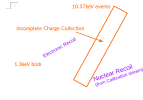
\includegraphics[width=\linewidth,]{Figures/Neutron/ecei_plot.png}
\caption{Reconstructed Ionization Energy in function of the Reconstructed Heat Energy, for the quality events of the Calibration configuration. The plot is zoomed up to 12keV for an easier view of the calibration peaks. }
\label{fig:ecei-plot}
\end{figure}

We recognize the noise blob near the origin corresponding to recoils of very low energy and triggering noise windows. Expanding from this noise blob, we note two bands. 
The electronic recoil band corresponds to events depositing the same energy in the ionization channel and the heat energy channel (both in keVee). They are characterized by a quenching factor of 1. As a matter of fact, the gamma recoil of 1.3keV and 10.37keV coming from the calibration peaks of the germanium belongs to this band. Any event below this band deposited less energy in the ionization channel than in the heat channel, and therefore possess a quenching factor inferior to one. We see that the population blob associated to the 10.37keV is smeared to lower quenching factor. This is due to events of the calibration peaks with incomplete charge collection. We note that this population is following a linear trend, which can be explained by an incomplete Luke-Neganov Boost of the heat channel according to the equation:
\begin{equation}
E_{heat} = 6 \textsf{keVee} + \epsilon \frac{2 \textsf{V}}{\epsilon_{Ge}} E_{ion.}
\end{equation}
The other major population of events below the electronic recoil band counts a lot of events in the case of the Calibration configuration. This hints that this band corresponds to the nuclear recoil induced by the AmBe neutron source.
The presence of the two bands in this plot demonstrate the discriminating ability of the associated heat and ionization channels. Note that, although the bands are well separated at high energy, they are merging at low energy due to their width which is fixed by the energy resolution of the heat and ionization channel.

Another way to represent the discrimination between the electronic and the nuclear recoil is to compute the recoil energy $E_R$ and the quenching factor $Q$ for each event:
\begin{align}
\label{eq:quenching-from-ecei}
	E_{NL} &= \frac{V}{\epsilon} ( E_{ion., ???} - E_{heat} )
	\\
	E_R = E_{heat} - E_{NL} &= E_{heat} \left( 1 + \frac{V}{\epsilon} \right) - E_{ion., ???} \frac{V}{\epsilon}
	\\
	Q &= \frac{E_{ion., ???}}{E_R}
\end{align}
with $E_{NL}$ being the heat energy boost coming from the Neganov-Luke effect \cite{luke-neganov-effect}.
The recoil energy $E_R$ is expressed in the usual $keV$ energy unit, as the Luke-Neganov Boost depending on the type of recoil was substracted from the heat energy. The Quenching factor is unitless.
The figure \ref{fig:quenching_plot} show, for each configuration, the quenching factor as a function of the recoil energy.

\begin{figure}
\centering
\includegraphics[width=\linewidth,]{Figures/Neutron/quenching_plot.png}
\caption{Quenching value $Q$ for each quality events of the Background (black) and Calibration (blue) configurations in function of their recoil energy $E_R$.}
\label{fig:quenching_plot}
\end{figure}

We recognize the electronic band, centered around $Q=1$ and the nuclear recoil band with $Q<0.4$. We also note some inter-band events like the smearing of the 10.37keV events hinting at the incomplete charge collection.

%HEAT ONLY EVENT
However, there are some interesting events with a quenching factor $Q=0$ which are known as "Heat-only" events. This population is infamously known in domains in the EDELWEISS experiment [ref?] and CRESST [ref?]. This population could correspond to events with no charge collection, but this is not compatible with the lower count of inter-band events with an incomplete charge collection. An other and more realistic explanation would be the existence of energy deposit in the crystal without ionization. The source of this Heat-only event is still under investigation [ref?].

The merging phenomenon of the bands at low energy is also more visible in this graph with the change of variable. We can even visually witness that the lower part of the 1.3keV event blob is leaking into the higher part of the nuclear band.


\subsection{Band cut}

With the obtainment of well reconstructed events, it is now time to count the events corresponding to electronic and nuclear recoils. The events will be allocated into different population based on their quenching factor and the resolution of the heat and ionization channel at the considered energies. This "band cuts" are represented on the figure \ref{fig:band-cut-ecei} with ionization and heat energies and on the figure \ref{fig:band-cut-quenching} by reasoning on the quenching factor and the recoil energy.

\begin{figure}
\centering
\includegraphics[width=\linewidth,]{Figures/Neutron/band_cut_ecei.png}
\caption{Band cut representation on the graph of Ionization energy vs Heat energy.}
\label{fig:band-cut-ecei}
\end{figure}

\begin{figure}
\centering
\includegraphics[width=\linewidth,]{Figures/Neutron/band_cut_quenching.png}
\caption{Band cut representation on the graph of Quenching vs Recoil Energy.}
\label{fig:band-cut-quenching}
\end{figure}

Electronic recoils are characterized by a quenching factor $Q_{ER}=1$. Nuclear recoil are associated to lower quenching factor depending on the recoil energy $E_R$ and the material of the absorber. According to the literature [Lindhard ref], with an atomic number of $Z=32$ and an average number of nucleons of $A=72.63$, the quenching factor of a nuclear recoil in a pure-germanium crystal is expressed as:
\begin{equation}
\label{eq:lindhard}
	Q_{NR}(E_R) = \frac{k g(E_R)}{1+k g(E_R)}
\end{equation}
with the $k,g$ terms calculated as:
\begin{align}
	k &= 0.133 Z^\frac{2}{3} A^\frac{-1}{2} \\
	\epsilon(E_R) &= 11.5 E_R Z^\frac{-7}{3} \\
	g(E_R) &= 3 \epsilon(E_R)^{0.15} + 0.7 \epsilon(E_R)^{0.6} + \epsilon(E_R) 
\end{align}
The heat-only event show a null quenching $Q_{HO}=0$.

These constraints on the quenching factor are translated in term of ionization and heat energy with the change of variables induced by eq \ref{eq:quenching-from-ecei}. For the electronic recoil, the ionization and heat energies follow:
\begin{align}
\label{eq:ER-char}
	E_{heat, ER} &= E_R \frac{1 + Q_{ER}\frac{V}{3}}{1 + \frac{V}{3}} = E_R \\
	E_{ion., ER} &= E_R Q_{ER} = E_R
\end{align}
The heat and ionization energy are theoretically equals.
For the neutron recoil, the energies follow:
\begin{align}
\label{eq:NR-char}
	E_{heat, NR} &= E_R \frac{1 + Q_{NR}(E_R)\frac{V}{3}}{1 + \frac{V}{3}} \\
	E_{ion., NR} &= E_R Q_{NR}(E_R)
\end{align}
As for the heat-only events, the energies are modeled as:
\begin{align}
\label{eq:HO-char}
	E_{heat, HO} &= E_R \frac{1 + Q_{HO}(E_R)\frac{V}{3}}{1 + \frac{V}{3}} = E_R \frac{1}{1 + \frac{V}{3}} \\
	E_{ion., HO} &= E_R Q_{HO}(E_R) = 0
\end{align}

An experimental event is allocated to the electronic recoil "ER" band if its ionization energy $E_{ion., exp}$ and heat energy $E_{heat, exp}$ follow the energy function associated to the ER recoil \ref{eq:ER-char} with a tolerance of two times the RMS resolution of the ionization energy at the considered heat energy, $\sigma_{ion}(E_{heat, exp})$. This condition to be satisfied is mathematically written as:
\begin{equation}
|E_{ion., exp} - E_{ion, ER}(E_{heat, exp})| < 2 \times \sigma_{ion}\left( E_{heat, exp}\right)
\end{equation}
Taking into account the equality of the heat and ionization energy in \ref{eq:ER-char}, this condition is also written as:
\begin{equation}
\label{eq:condition-ER-ecei}
|E_{ion., exp} - E_{heat_exp}| < 2 \times \sigma_{ion}\left( E_{heat, exp}\right)
\end{equation}

Concerning the allocation in the neutron recoil "NR" band, the heat and ionization energies should now follow the functions associated to the neutron recoil \ref{eq:NR-char}. The tolerance is still fixed to two times the RMS resolution $\sigma_{ion}(E_{heat, exp})$. The condition now is expressed as:
\begin{equation}
\label{eq:condition-NR-ecei}
|E_{ion., exp} - E_{ion, NR}(E_{heat, exp})| < 2 \times \sigma_{ion}\left( E_{heat, exp}\right)
\end{equation}
One should note that according to the expressions \ref{eq:NR-char}, their is no analytical expression of the ionization energy $E_{ion, NR}$ as a function of the heat energy. To bypass this issue, $E_{ion, NR}$ is computed over a fine array of heat energy between 0keV and 50keV. The term $E_{ion, NR}(E_{heat, exp})$ is therefore obtained by linear interpolation.

As for the allocation to the heat-only "HO" band, we use the modelization of the heat-only event energies in equations \ref{eq:HO-char} to define the condition:
\begin{equation}
|E_{ion., exp} - E_{ion, HO}(E_{heat, exp})| < 2 \times \sigma_{ion}\left( E_{heat, exp}\right)
\end{equation}
which is simplified to:
\begin{equation}
\label{eq:condition-HO-ecei}
|E_{ion., exp}| < 2 \times \sigma_{ion}\left( E_{heat, exp}\right)
\end{equation}

The ER, NR and HO band defined by the three previous conditions \ref{eq:condition-ER-ecei}, \ref{eq:condition-NR-ecei} and \ref{eq:condition-HO-ecei} respectively are represented on the figure \ref{fig:band-cut-ecei} along with the experimental events passing the quality cuts. With the change of variable \ref{eq:quenching-from-ecei}, the ER, NR and HO bands are also defined in terms of quenching factor and recoil energy in figure \ref{fig:band-cut-quenching}. 
It is now possible to obtain a raw recoil energy spectrum of the different bands by counting the number of events in each energy bins. These histograms are presented in figure \ref{fig:raw-hist}.

\begin{figure}
\centering
\includegraphics[width=\linewidth,]{Figures/placeholder}
\caption{Histogram of the event allocated to the ER, NR and HO bands in function of their recoil energy.}
\label{fig:raw-hist}
\end{figure}

We can note some usual features in this histogram like the noise blob at the lowest energies, the 1.3keV events and the 10.37keV of the calibration peaks. As before, we see that from 6keV and below, the different bands are merging into each other. The lower parts of the 1.3keV and 10.37keV population of the calibration peaks are even counted in the NR and HO band !
This contamination between the bands is harmful for an unbiased counting of the events in each bands.
Moreover, the experimental events presented in the figures were the one passing the quality cuts presented previously. Even though this cuts were vital to prune the data from ill-reconstructed events, they effectively reduced the number of events in the ER, NR and HO bands, which are therefore underestimating the initial number of recoils having happened.


\subsection{Energy spectrum correction}

In order to estimate the true ER, NR and HO background, it is necessary to correct the raw histograms \ref{fig:raw-hist} from the following bias:
\begin{itemize}
	\item the efficiency of the quality cuts, to take into account all the events which did not passed the quality cuts
	\item the cross-band contamination, particularly at the lowest energy when the bands are merging
\end{itemize}
In this analysis, we choose to use a method called "Pulse Simulation" to estimate these bias.


\subsubsection{Pulse simulation}

This method aims at simulating signals (aka pulses) of ER and NR recoil with known recoil energy and injecting them into the experimental stream. Thus, this technique is only valid when the whole stream of data is saved. All the steps of the pulse simulation described in this very section were realized by Julien Billard.

The simulation of a signal comes from a bank of well characterized events. This bank is built with a selected population of 10.37keV event from the associated calibration peak passing the quality cuts as represented in the figure \ref{fig:ecei-plot}. These selected events comes from gamma recoils with a known recoil energy. Although most of these events present a complete charge collection associated with a quenching $Q_{ER}=1$, some are subjects to incomplete charge collection (and still taken into account ??? are discarded ??? idk).

Once the bank of 10.37keV events is formed, we proceed with the the simulation of events coming from ER and NR recoil and with the wanted recoil energy. We fix the recoil energy of a simulated event by scaling the signal of the 10.37keV event from the bank with a rule of three. Simulating event coming from electronic recoil is straightforward as the 10.37keV event of the bank are already produced by gamma recoils. As for the simulation of events coming from nuclear recoil, the ionization and heat energies should be corrected to present a quenching calculated from the Linhard formula in equation \ref{eq:lindhard}.

In this analysis, four different population of events were simulated:
\begin{itemize}
	\item 10.37keV line ER events: the most straightforward simulation as these simulated corresponds to the raw selected events of the bank.
	\item 1.3keV line ER events: simply rescaling the bank of events provides this simulated population corresponding to the second calibration peak of the germanium.
	\item $[0-50]$keV flat ER events: this uniform distribution in recoil energy is obtained by rescaling the bank of events by radom factors.
	\item $[0-50]$keV flat NR events: as before, this is a uniform distribution in recoil energy and corrected in heat and ionization energy to present an appropriate quenching factor $Q_{NR}$.
\end{itemize}

The pulse simulation continues with the injection of these simulated population into the saved streams. This means taking one event of a population, and adding it to stream at a random known time $t_0$. In order to keep this probing technique from altering too much the characteristics of the analysis, it is decided to inject a maximum of 60(?) pulses per hour of streams. This process is repeated multiples times with different $t_0$ and for the four simulated population independently.

An important remark is to be made here concerning the signal noise injected in the streams along with the simulated pulses. The 10.37keV events composing the bank of events and used for the creation of the simulated population are real events from the streams affected a signal noise. By adding simulated pulses to the streams, we are effectively adding the noise of the simulated pulse and the noise of the stream. This means that all the pulses that are injected into the streams are by construction noisier than real pulses.
While the effect of this phenomenon is negligible at low energies as the 10.37kev and its associated noise were scaled down, for higher energies this additional noise might result in a worse energy reconstruction than real pulses as well as lead to a discarding by the $\chi^2$ cut.
As a concrete example, an injected pulse of the "10.37keV line ER" population should be affected by a noise PSD with a factor $\sqrt{2}$ higher than the noise PSD of a real 10.37keV pulses of the stream. This will result in a biased $\chi^2$ value for the simulated pulse, sampled from a $\chi^2$ distribution of mean $\sqrt{2}N$ rather than $\sqrt{N}$. Hopefully, the $\chi^2$ cut of this analysis (presented in \ref{par:quality-cuts}) are large enough to alleviate this effect. As for the energy reconstruction, the bias should be covered by the energy resolution of the sensors.
Having considered the existence of this added noise, we can considered that the simulated pulse are excellent facsimiles of the real pulses with the major advantages than we know their input recoil energy $E_R^{input}$, their injection time $t_0^{input}$ and their quenching $Q_{ER}$ or $Q_{NR}(E_R^{input})$ (depending on the simulated population they belong to.



\subsubsection{Trigger cut}

{\color{red} this explanation definitively needs a plot to explanation all the different cases and the different t0, else this will be too much confusing :(}

Just as in the previous section \ref{par:data-format}, the newly created streams with injected pulses are pre-processed using optimal filtering and information on the triggering time windows are saved.
As what is interesting us in this streams are the injected pulses, we are focusing on the triggering events.
The objective is this section is to decide whether a simulated event injected at $t_0^{input}$ has properly triggered or not.
On the one hand, we should discard "non-triggering" simulated event where:
\begin{itemize}
	\item the simulated pulse with a low energy could not have reach the trigger threshold, and the an earlier or later real triggering pulse was selected as closest to the injection time $t_0^{input}$
	\item a simulated pulse could have been injected near (<0.5s) a real pulse of higher energy. As both the simulated and the real pulses are triggering and are close in time, only the real one with the highest reconstructed energy is triggering.
\end{itemize}
A maximum tolerance of $5$ms between the injection time of a simulated pulse $t_0^{input}$ and the timestamp of the closest triggering event $t_0$ was arbitrary chosen to ensure that the triggering pulses are in fact corresponding to simulated pulses.
On the other hand, a triggering simulated event could also have been injected exactly at the same time as a real pulse of the stream, this occurrence is called a "pile-up". The resulting signal is the addition of a real and the injected pulse which will bias the energy reconstruction. A minimum time of $5$ms between the timestamp of the closest triggering event $t_0^{input}$(extracted from the stream with injected simulated pulses) and the timestamp of the closest triggering real pulse $t_0^{data}$(extracted from the original stream) was chosen to discard any pile-up event.
By combining this two condition ensuring a proper triggering of the simulated event, we can define the "trigger cut" condition:
\begin{equation}
\left\{
\begin{array}{r c l}
| t_0^{input} - t_0 | &\geq& 5\textsf{ms}\\
| t_0 - t_0^{data} | &\leq& 5\textsf{ms}
\end{array}
\right.
\end{equation}
Triggering event of timestamp $t_0$ closest to a $t_0^{input}$ satisfying this condition are considered as having properly triggered.

It is important to note that this trigger cut is specific to simulated pulses. In order to reproduce such a study with real pulses can only be done if we know the exact time of the energy deposit in the crystal. Access to this piece of information is impossible in this work using either an AmBe neutron source or the gamma calibration peak of the germanium as both this source are based on the intrinsically stochastic process of radioactive decay. However, the use of controlled source of particles could be envisioned:
\begin{itemize}
	\item facing the germanium crystal inside the cryostat, an optical fiber linked to a pulsing LED could be used as a repetitive source of electronic recoil.
	\item outside of the cryostat, a pulsed neutron source would be overkill (or would it ? idk just thinking here)
\end{itemize}

Now that we have selected the simulated pulses which properly triggered, the entire analysis chain of this very chapter \label{ChapterNeutron} described until now is applied to these events. The triggering simulated events population is pruned of the reconstruction biased with the quality cuts and are then allocated to the ER, NR and HO bands.

\subsubsection{Band Contamination Correction}

\subsubsection{Efficiency cut correction}

Trigger cut: Livetime and Pile-up

Quality cuts should be the broad term for all the cuts before band...







